\documentclass{article}

\usepackage{amsmath}
\usepackage{fullpage}
\usepackage{url}
\usepackage{xspace}


\title{Examples of how to use functions}
\author{Kwame Okrah, Hector Bravo}
\date{\today}

\usepackage{Sweave}
\begin{document}
\Sconcordance{concordance:example.tex:example.Rnw:%
1 12 1 1 0 34 1 1 2 1 0 1 2 1 0 2 1 18 0 1 1 5 0 2 1 6 0 1 2 2 1 1 6 5 %
0 1 1 13 0 1 2 2 1 1 3 2 0 1 3 2 0 1 2 1 0 1 1 5 0 2 1 1 4 6 0 1 2 2 1 %
1 2 13 0 1 2 1 1 1 6 5 0 1 1 4 0 1 2 12 1 1 4 13 0 1 1 5 0 1 1 1 2 1 0 %
1 2 13 0 1 7 5 0 1 1 4 0 1 2 1 1 1 2 5 0 2 2 49 0 3 1 3 0 2 2 1 0 1 2 1 %
0 3 1 4 0 1 2 1 1 1 2 1 0 1 1 1 2 1 0 4 1 3 0 2 2 1 0 1 1 10 0 1 2 4 1}

\maketitle

\section{Overview of pipeline}
The purpose of this pipeline is to streamline the process for analyzing RNA-seq data
with potential batch effects. The pipeline includes 1) quantile normalization 2) log-transformation of counts 3) combat (location) batch correction 4) voom calculation of weights.\\\\
The functions in this package can be grouped into two main categories:

\begin{enumerate}
\item The functions used for assessing batch effects.
    \begin{itemize}
    \item makeSVD
    \item pcRes
    \item plotPC
    \end{itemize}
\item The functions for removing batch effect and computing weights for limma.
    \begin{itemize}
    \item qNorm
    \item log2CPM
    \item voomMod
    \item combatMod
    \item batchSEQ$^*$
    \end{itemize}
\end{enumerate}
$^*$ batchSEQ is the pipeline function. It combines qNorm, log2CPM, voomMod, and combatMod
into one step.\\\\
Below we will illustrte how to use these functions using the pasilla data set.\\\\
{\bf note}: All the functions in this package have a detailed help file which tells you
what kind of objects go in and what kind of objects come out. It is important to look
at these help files for each function.

\section{Examples of how to use the functions}
We will use the pasilla dataset found in the pasilla package. (This is the same dataset used
in the DESeq vignette)
\begin{Schunk}
\begin{Sinput}
> require(pasilla)
> # locate the path of the dataset and read in the dataset
> datafile = system.file("extdata/pasilla_gene_counts.tsv", package="pasilla")
> counts = read.table(datafile, header=TRUE, row.names=1)
> head(counts)
\end{Sinput}
\begin{Soutput}
            untreated1 untreated2 untreated3 untreated4 treated1 treated2
FBgn0000003          0          0          0          0        0        0
FBgn0000008         92        161         76         70      140       88
FBgn0000014          5          1          0          0        4        0
FBgn0000015          0          2          1          2        1        0
FBgn0000017       4664       8714       3564       3150     6205     3072
FBgn0000018        583        761        245        310      722      299
            treated3
FBgn0000003        1
FBgn0000008       70
FBgn0000014        0
FBgn0000015        0
FBgn0000017     3334
FBgn0000018      308
\end{Soutput}
\begin{Sinput}
> dim(counts)
\end{Sinput}
\begin{Soutput}
[1] 14599     7
\end{Soutput}
\begin{Sinput}
> counts = counts[rowSums(counts) > ncol(counts),]
> dim(counts)
\end{Sinput}
\begin{Soutput}
[1] 10153     7
\end{Soutput}
\end{Schunk}
In this dataset there are two biological conditions: treated (3 samples) and untreated (4 samples). 
Two samples are single-end and the other 4 are paired-end. We will use sigle-end and paired-end
as bathch effects. Below is the design (pheno data.frame).
\begin{Schunk}
\begin{Sinput}
> design = data.frame(row.names=colnames(counts), 
+                     condition=c("untreated","untreated","untreated",
+                                 "untreated","treated","treated","treated"),
+                     libType=c("single-end","single-end","paired-end",
+                               "paired-end","single-end","paired-end","paired-end"))
> design
\end{Sinput}
\begin{Soutput}
           condition    libType
untreated1 untreated single-end
untreated2 untreated single-end
untreated3 untreated paired-end
untreated4 untreated paired-end
treated1     treated single-end
treated2     treated paired-end
treated3     treated paired-end
\end{Soutput}
\end{Schunk}
\subsection{Explore data for batch effects}
We will begin our analysis by exploring the data for possible/significant batch effects.

\begin{Schunk}
\begin{Sinput}
> # load batch package
> require(cbcbSEQ)
> #
> # quantile normalize: adjust counts for library size.
> qcounts = qNorm(counts)
> # convert counts to log2 counts per milliom. (voom scale)
> cpm = log2CPM(qcounts)
> names(cpm)
\end{Sinput}
\begin{Soutput}
[1] "y"        "lib.size"
\end{Soutput}
\begin{Sinput}
> libsize = cpm$lib.size
> cpm = cpm$y
> #
> # PCA analysis
> # returns a list with two components v and d.
> res = makeSVD(cpm)
\end{Sinput}
\end{Schunk}
We can now call pcRes and plotPC.
\begin{itemize}
\item pcRes: computes variance of each principal component and how they "correlate" with batch and condition.\\\\
\begin{Schunk}
\begin{Sinput}
> pcRes(res$v,res$d, design$condition, design$libType)
\end{Sinput}
\begin{Soutput}
  propVar cumPropVar cond.R2 batch.R2
1   27.57      27.57   48.13    67.00
2   24.66      52.23   50.74    31.82
3   15.62      67.85    0.57     0.04
4   12.15      80.00    0.05     0.35
5   10.53      90.53    0.14     0.14
6    9.46      99.99    0.37     0.65
\end{Soutput}
\end{Schunk}
\item plotPC: Plot first 2 principal components. This function works like the regular plot function in R. ie. We can add all the options to make the plot sensible and well labelled. Below is an 
example:
\begin{Schunk}
\begin{Sinput}
> plotPC(res$v,res$d, 
+        col=design$condition, # color by batch
+        pch=19, main="PCA plot",
+        xlim=c(min(res$v[,1])-.08,max(res$v[,1])+.08),
+ 	     ylim=c(min(res$v[,2])-.08,max(res$v[,2])+.08))
> text(res$v[,1], res$v[,2], design$libType, pos=1, cex=0.6) 
\end{Sinput}
\end{Schunk}
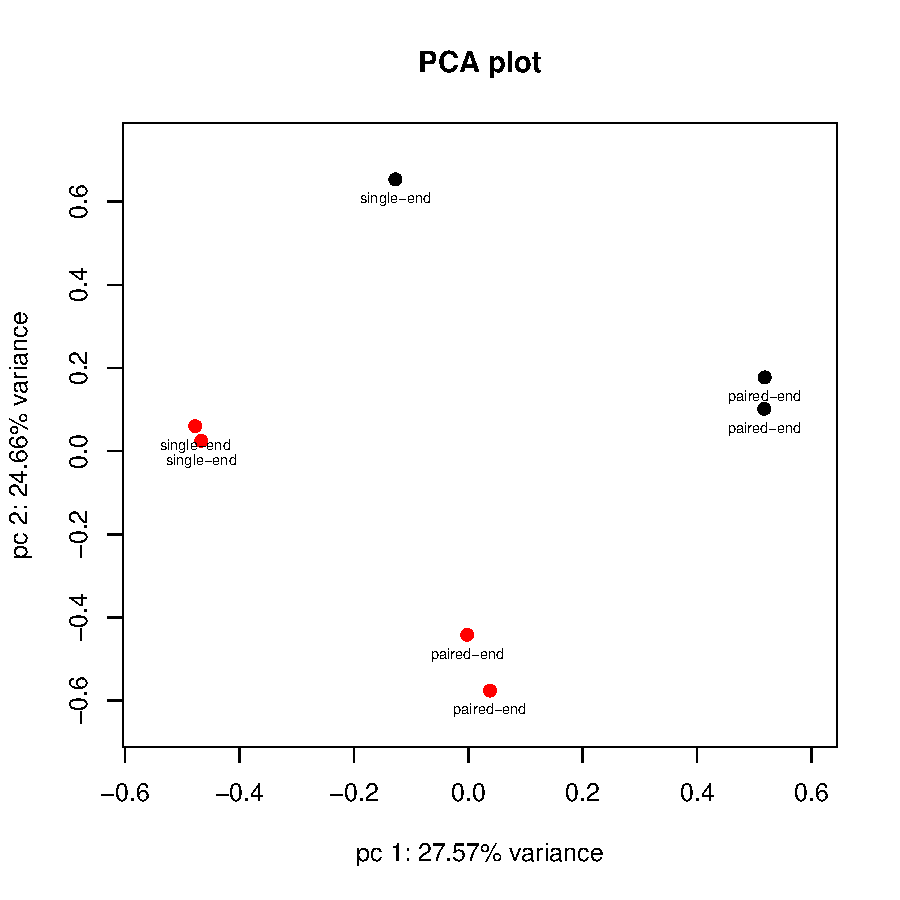
\includegraphics{example-005}
\end{itemize}

We see that there is a batch effect in the data. Both in the PCA "correlation" table
and the PCA plot.
\subsection{Correct data for batch effects}
The standard way to correct for batch effects will be to account for batch in the linear
model. However we will use a modified version of combat instead. 
In this only adjust batch location. We do not adjust for scalar batch effects.
This is because the data is not necessarily Gaussian. In order to account for scaling
we have to take into account the mean var relationship inherent in this kind of data.
We adjust batch location by removing the empirical beysian estimates of batch effects.
(Future work)

\begin{Schunk}
\begin{Sinput}
> # combatMod function
> # noScale=TRUE option not to scale adjust
> tmp = combatMod(cpm, batch=design$libType, mod=design$condition, noScale=TRUE)
\end{Sinput}
\begin{Soutput}
Found 2 batches
Found 1  categorical covariate(s)
Standardizing Data across genes
Fitting 'shrunk' batch 1 effects
Fitting 'shrunk' batch 2 effects
Adjusting data for batch effects
\end{Soutput}
\begin{Sinput}
> names(tmp)
\end{Sinput}
\begin{Soutput}
[1] "bayesdata" "info"     
\end{Soutput}
\begin{Sinput}
> tmp = tmp$bayesdata
> # look at PCA results again
> res = makeSVD(tmp)
> # batch effect is reduced
> pcRes(res$v,res$d, design$condition, design$libType)
\end{Sinput}
\begin{Soutput}
  propVar cumPropVar cond.R2 batch.R2
1   30.97      30.97   99.00     2.71
2   18.65      49.62    0.47     0.80
3   14.69      64.31    0.02     5.89
4   12.65      76.96    0.04    10.40
5   12.09      89.05    0.30    46.56
6   10.94      99.99    0.18    33.64
\end{Soutput}
\end{Schunk}
\begin{Schunk}
\begin{Sinput}
> plotPC(res$v,res$d, 
+        col=design$condition, # color by batch
+        pch=19, main="PCA plot",
+        xlim=c(min(res$v[,1])-.08,max(res$v[,1])+.08),
+        ylim=c(min(res$v[,2])-.08,max(res$v[,2])+.08))
> text(res$v[,1], res$v[,2], design$libType, pos=1, cex=0.6) 
\end{Sinput}
\end{Schunk}
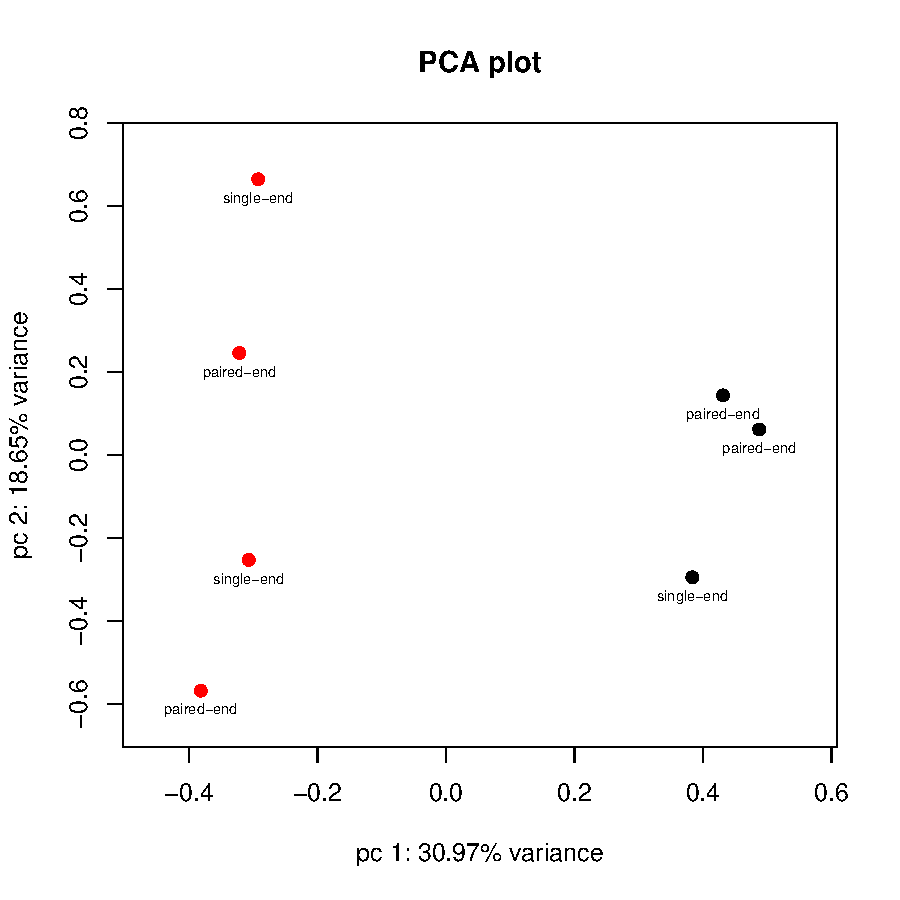
\includegraphics{example-007}
We are now ready to use limma. However we must compute the weights. We modify so
it does not assume that the data are counts.
\begin{Schunk}
\begin{Sinput}
> v = voomMod(tmp, model.matrix(~design$condition), lib.size=libsize, plot=TRUE)
\end{Sinput}
\end{Schunk}
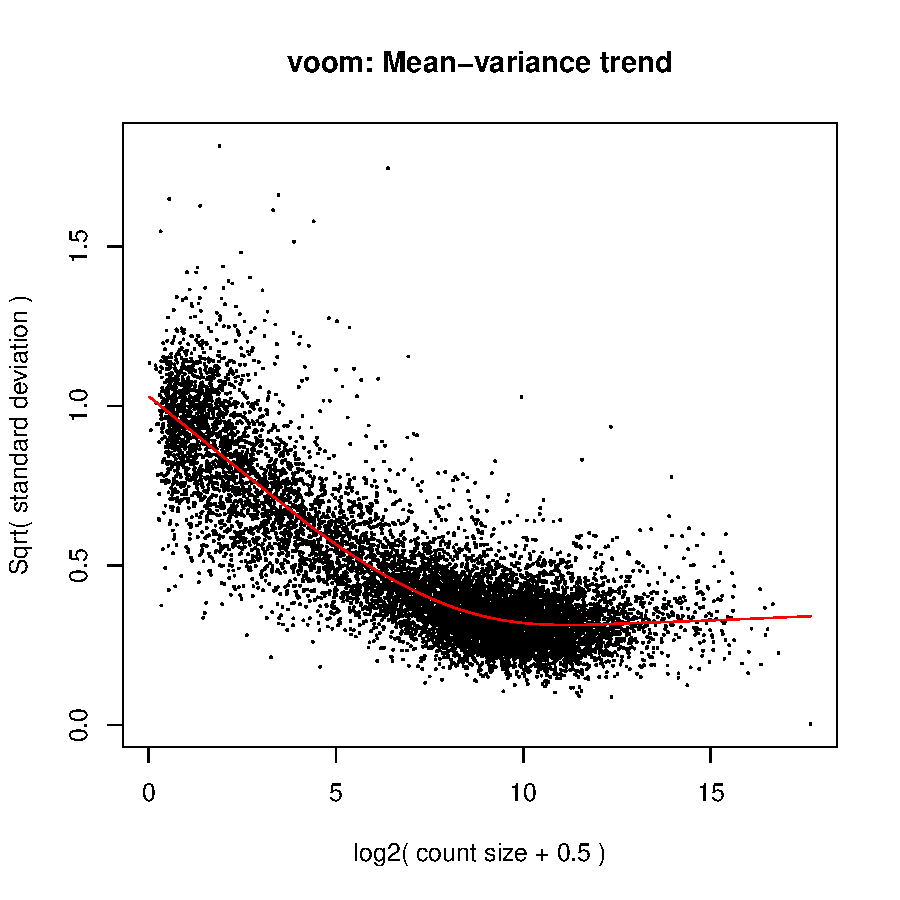
\includegraphics{example-008}

\begin{Schunk}
\begin{Sinput}
> v
\end{Sinput}
\begin{Soutput}
An object of class "EList"
$E
            untreated1 untreated2 untreated3 untreated4  treated1   treated2
FBgn0000008  2.9772407  3.0375781   3.259578   2.852434  2.847232  3.1729673
FBgn0000014 -1.2338011 -4.2500923  -3.970097  -3.970114 -2.500071 -3.9701281
FBgn0000017  8.3918375  8.6390002   8.703652   8.391730  8.373702  8.3253415
FBgn0000018  5.2548863  5.0144051   5.067631   5.157916  5.045165  5.1067903
FBgn0000024 -0.3373151 -0.9737137  -1.280256  -1.320351 -1.124131 -0.2509431
              treated3
FBgn0000008  2.7072849
FBgn0000014 -3.9701469
FBgn0000017  8.3401799
FBgn0000018  5.0125956
FBgn0000024 -0.8702176
10148 more rows ...

$weights
          [,1]      [,2]      [,3]      [,4]       [,5]        [,6]        [,7]
[1,] 26.520373 26.520219 26.519769 26.520017  24.814440  24.8144274  24.8146913
[2,]  1.017667  1.017662  1.017650  1.017657   0.970376   0.9703756   0.9703826
[3,] 99.583486 99.583548 99.583731 99.583630 100.681377 100.6813824 100.6812770
[4,] 71.619883 71.619617 71.618838 71.619267  69.924363  69.9243415  69.9247981
[5,]  2.838734  2.838720  2.838677  2.838700   3.176932   3.1769302   3.1769600
10148 more rows ...

$design
  (Intercept) design$conditionuntreated
1           1                         1
2           1                         1
3           1                         1
4           1                         1
5           1                         0
6           1                         0
7           1                         0
attr(,"assign")
[1] 0 1
attr(,"contrasts")
attr(,"contrasts")$`design$condition`
[1] "contr.treatment"


$lib.size
untreated1 untreated2 untreated3 untreated4   treated1   treated2   treated3 
  13237697   13237599   13237313   13237471   13237605   13237597   13237770 
\end{Soutput}
\begin{Sinput}
> fit = lmFit(v)
> eb = eBayes(fit)
> top = topTable(eb, coef=2, n=nrow(v$E))
\end{Sinput}
\end{Schunk}
Plot results
\begin{Schunk}
\begin{Sinput}
> sel = top$adj.P.Val < 0.05
> plot(top$logFC, -log10(top$adj.P.Val), pch=16, cex=0.3,
+      main=paste(sum(sel), "/", length(sel)))
> sel = top$adj.P.Val < 0.05
> points(top$logFC[sel], -log10(top$adj.P.Val)[sel], col="red", cex=0.3)
> abline(v=c(-1,1), h=-log10(0.05), col="blue")
\end{Sinput}
\end{Schunk}
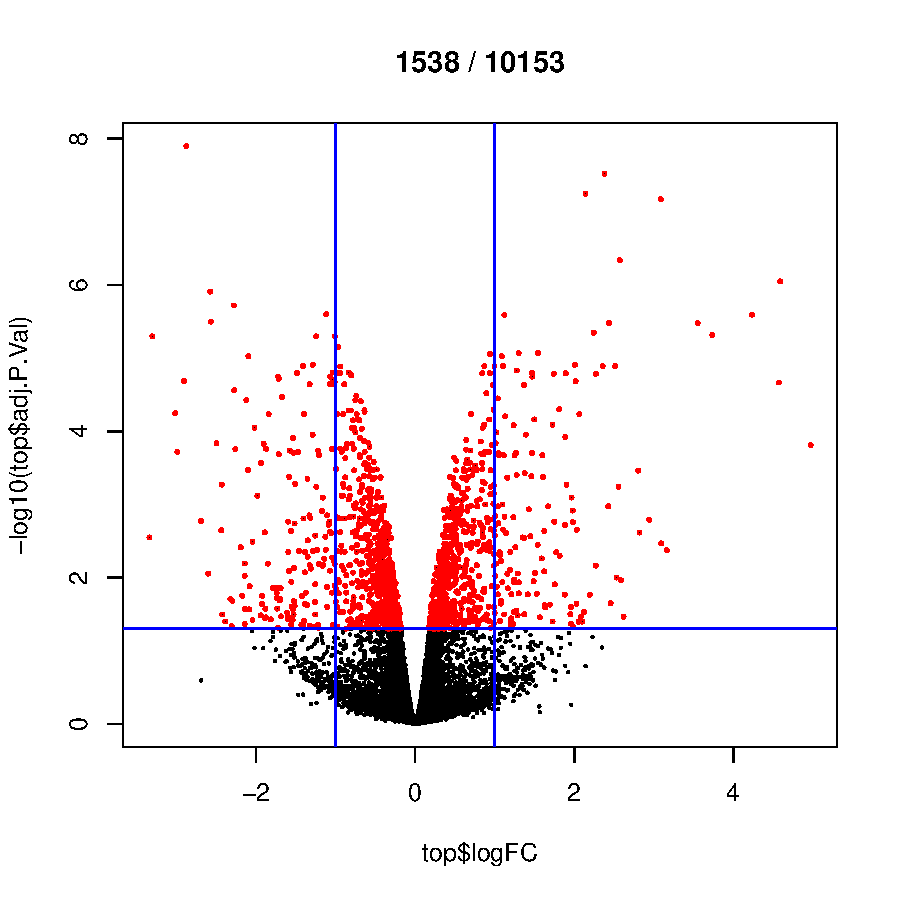
\includegraphics{example-010}
Let us now compare the results to what we get when we adjust for bath in the model

\begin{Schunk}
\begin{Sinput}
> cond=design$condition
> batch=design$libType
> mod = model.matrix(~cond+batch ,
+                    contrasts.arg=list(cond="contr.treatment", batch="contr.sum"))
> v1 = voom(counts, mod) 
> fit1 = lmFit(v1)
> eb1 = eBayes(fit1)
> top1 = topTable(eb1, coef=2, n=nrow(v1$E))
\end{Sinput}
\end{Schunk}
Compare results results:
\begin{Schunk}
\begin{Sinput}
> tab = merge(top[,c("ID", "adj.P.Val")], top1[,c("ID", "adj.P.Val")], by="ID")
> as.data.frame(table(combat = tab[,2] < 0.05, model = tab[,3] < 0.05))
\end{Sinput}
\begin{Soutput}
  combat model Freq
1  FALSE FALSE 8516
2   TRUE FALSE  401
3  FALSE  TRUE   99
4   TRUE  TRUE 1137
\end{Soutput}
\end{Schunk}
We gain slightly more with combat.



\end{document}
